
%%%%%%% GPUs: Disillusion %%%%%%%

\begin{frame}[fragile]
\frametitle{GPUs: Disillusion}
 \begin{block}{Computing Architecture Schematic}
  \begin{center}
   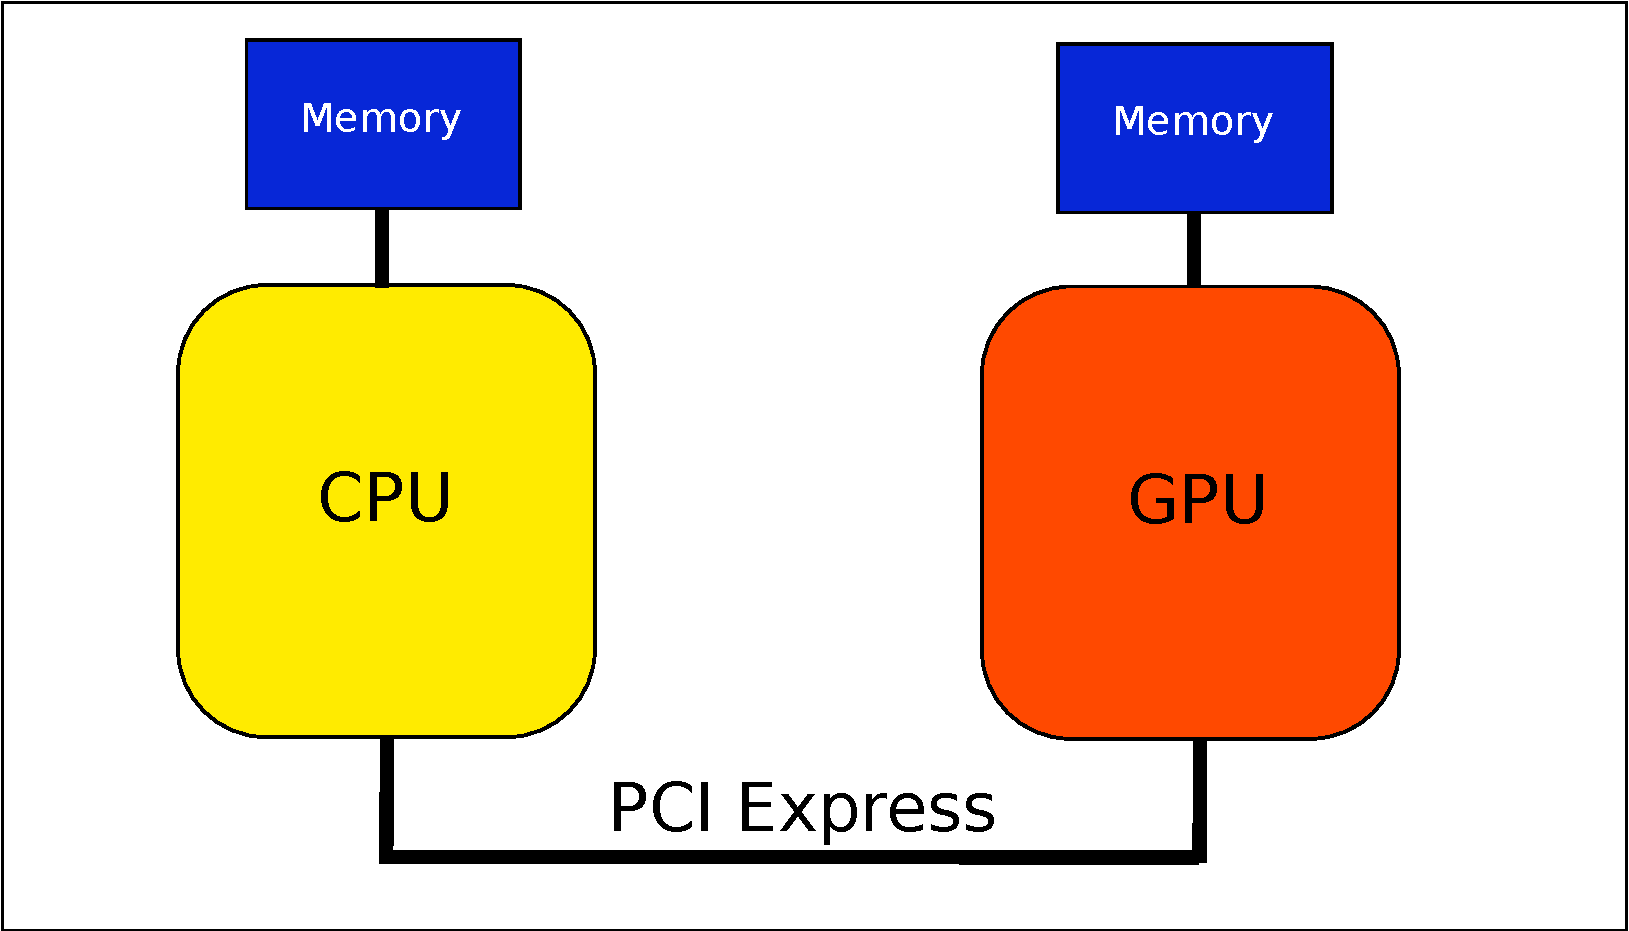
\includegraphics[width=0.8\textwidth]{figures/cpu-gpu-coarse.pdf}
  \end{center}

 
 \begin{itemize}
  \item \vspace*{1.03cm}
 \end{itemize}
 \end{block}

\end{frame}

\begin{frame}[fragile]
\frametitle{GPUs: Disillusion}
 \begin{block}{Computing Architecture Schematic}
  \begin{center}
   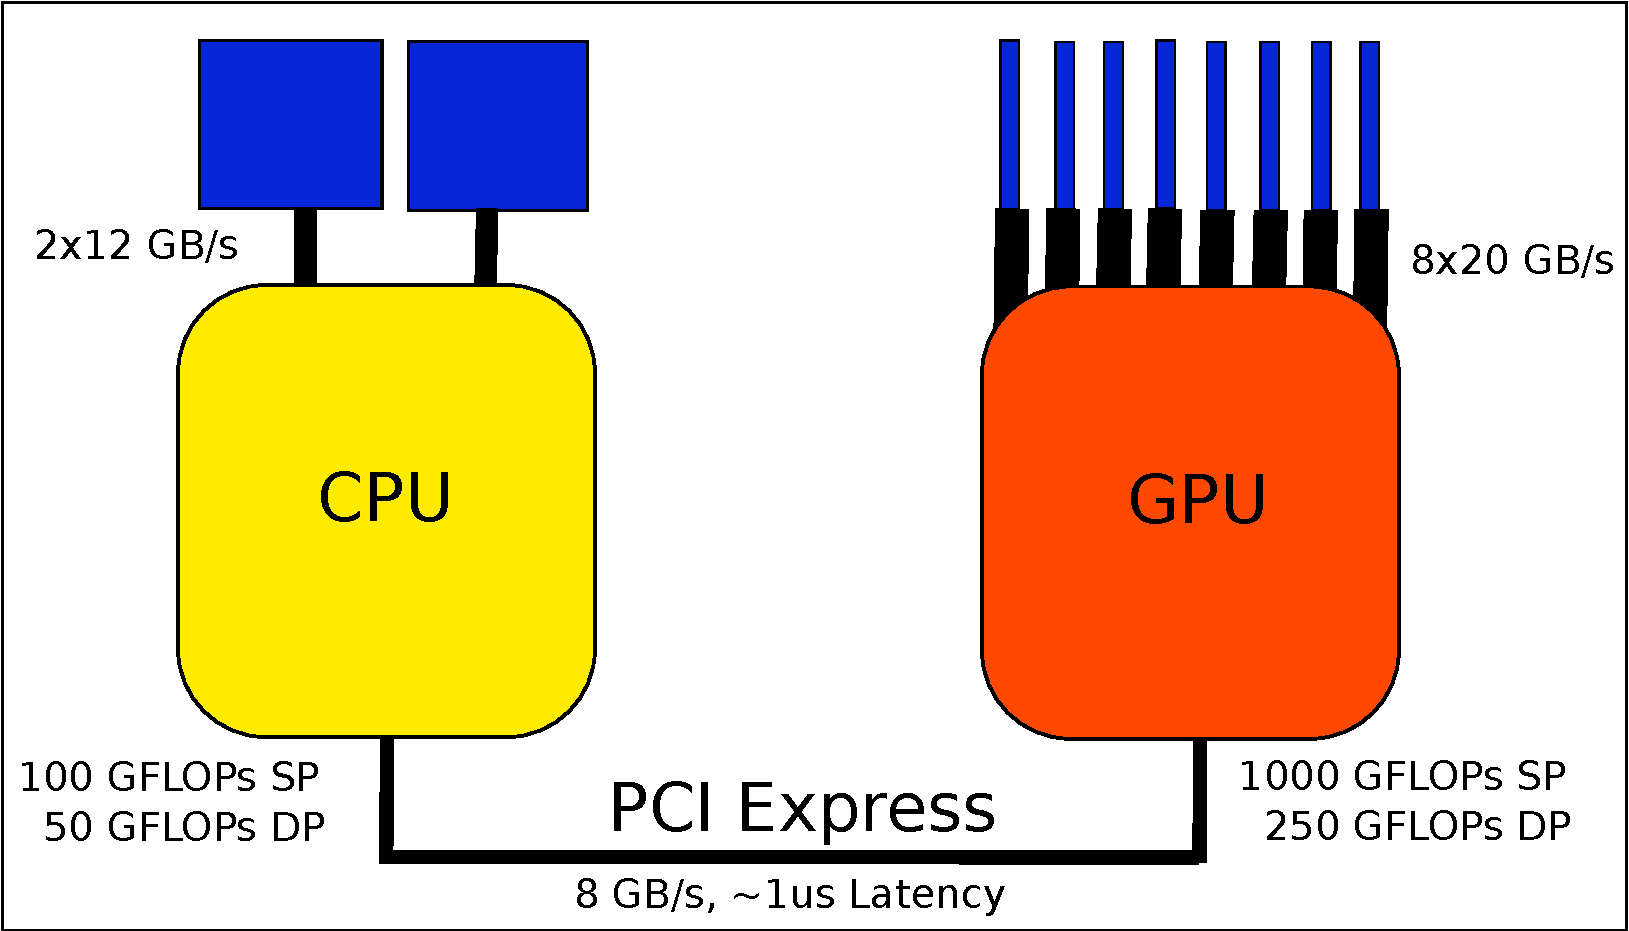
\includegraphics[width=0.8\textwidth]{figures/cpu-gpu-detail.pdf}
  \end{center}

 \begin{itemize}
  \item Good for large FLOP-intensive tasks, high memory bandwidth
  \item PCI-Express can be a bottleneck
  \item $\gg 10$-fold speedups (usually) not backed by hardware
 \end{itemize}
 \end{block}

\end{frame}



\begin{frame}{GPU Programming Approaches}
 
  \begin{block}{CUDA}
   \begin{itemize}
   \item Almost no additional code required
   \item Vendor-lock
   \item Relies on \lstinline|nvcc| being available
  \end{itemize}

  \end{block}

  \begin{block}{OpenCL}
  \begin{itemize}
   \item Additional boilerplate code required (low-level API)
   \item Broad hardware support (separate SDKs)
   \item No more development effort from NVIDIA
  \end{itemize}
  \end{block}

  \begin{block}{Directives}
   \begin{itemize}
    \item Annotate existing code with OpenMP-style Pragmas
    \item OpenACC and others
   \end{itemize}

  \end{block}

\end{frame}


\begin{frame}[fragile]{PETSc GPU Support}
 
  \begin{block}{NVIDIA Cusp/Thrust/CUSPARSE}
   \begin{itemize}
   \item Compile PETSc with CUDA support
   \item Use command line options to enable types, e.g.
    \begin{lstlisting}
 -vec_type cusp -mat_type aijcusp
    \end{lstlisting}
  \end{itemize}
  \end{block}

  \begin{block}{ViennaCL (OpenCL)}
  \begin{itemize}
   \item Compile PETSc with OpenCL support
   \item Use command line options to enable types, e.g.
    \begin{lstlisting}
 -vec_type viennacl -mat_type aijviennacl
    \end{lstlisting}
   \item Used for subsequent benchmarks
  \end{itemize}
  \end{block}

 \begin{center} No change in application code required! \end{center}
                                                        
\end{frame}


\begin{frame}{Benchmarks}
  \begin{center}
   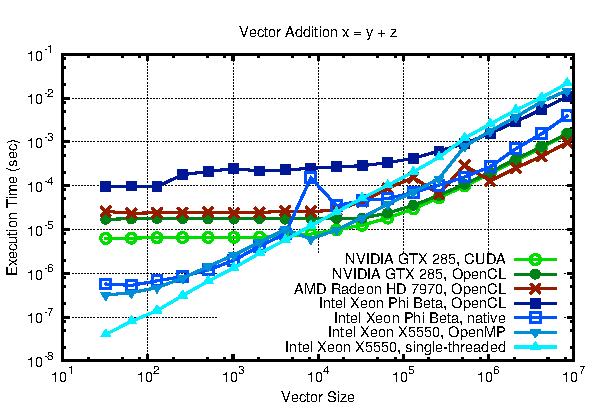
\includegraphics[width=0.95\textwidth]{figures/vector-timings-7}
  \end{center}
\end{frame}

%%


\begin{frame}{Benchmarks}
  \begin{center}
   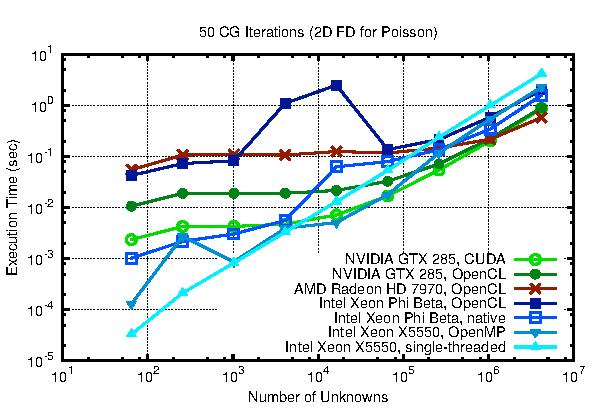
\includegraphics[width=0.95\textwidth]{figures/cg-timings-7}
  \end{center}
\end{frame}

